\chapter{Lambda Architecture}
\label{chap:lambda_architecture}

The Lambda architecture \cite{MarzWarren201401} is a new solution
for creating a BigData system of any type. It provides the model for scalable,
fault-tolerant, distibuted processing of data. It uses both batch and online
processing to answer the queries. It provides human fault-tolerance, what is
often overlooked in other approaches. The Lambda architecture lets developer to
concentrate on the bussiness-logik, instead of thinking about distributing
computations, replication of dataset and how to manage intense grow of input data.

The core of the Lambda architecture is the equation "query = function(all
data)". The idea is that to answer any kind of query one can take the whole
dataset and execute particular function. The problem is that it is unreasonably
expensive, and even infeasible in most of cases. To solve this issue one can
create views, that are helpful for answeing particular queries, in advance. The
only problem of such approach is that indexing all the data and creating views
is high-latency operation. It can take several hours to be done. To overcome
this delay the Lambda architecture provides online processing of the data coming
in the real-time, that has not yet appeared in the precomputed views. As a
result, to answer the query both things are used: views, computed on the whole
dataset in advance, and sketch of the very new data.

One key aspect of the Lambda architecture, that makes a difference with the
other approaches, is that human fault-tolerance is concerned inherently. This is
important issue, because mistakes in programming code are guarantied. And as a
result, deleting or updating the data in a wrong way is also possible. The Lambda
architecture doesn't allow to modify data. This is called \mnote{Immutability}
immutability. Data can be only added, and never can be deleted or updated. This
leads to completely different model of storing data. Instead of having simple
tuple for a particular entity, every value of a tuple is stored separately and
has timestamp. Such technique allows to have the whole history of editions of
all attributes, what can be useful to make quesries that use history of changes.
At the same time the actual value is the one with the oldest timestamp.

\authorsection{General structure}{VI}

General view of the Lambda architecture is depicted on the
Figure~\ref{fig:lambda_architecture}. It consists of three main elements: batch
layer, serving layer and speed layer. Batch layer contains master dataset, that
allows only appending data. One executes computations on the whole master
dataset to obtain batch views, that are useful to answer queries. Serving
layer is the place where batch views are stored. It is also responsible for
providing interface for making particular queries from those views. Speed layer
provides temporal views. They contain sketches of data, that was obesrved during
ongoing batch processing in the batch layer. It is important, because batch
processing can last several hours or even longer. Speed layer is much more
complex than batch layer, and it provides only approximated results. We discuss
it in more details in the particular chapter.

\begin{figure}[H]
  \centering
  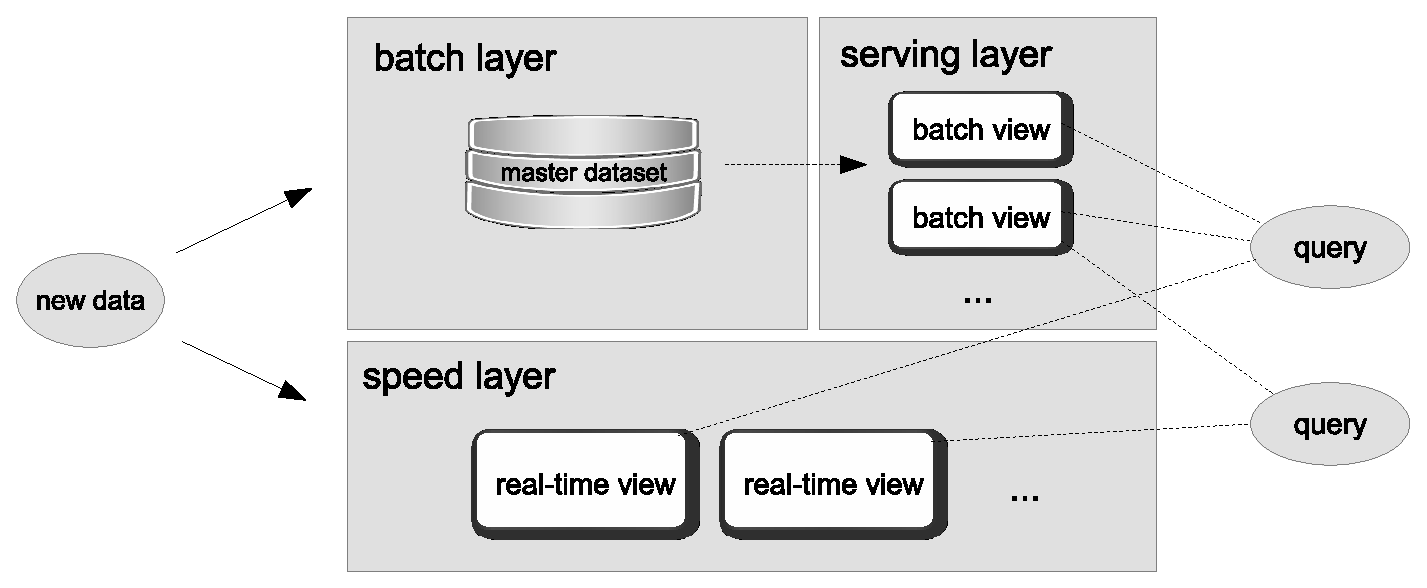
\includegraphics [width=0.9\textwidth]{images/LambdaArchitecture}
  \caption{General structure of the Lambda architecture}
  \label{fig:lambda_architecture}
\end{figure}

\authorsection{Batch layer}{VI}

Batch layer is the part of the Lambda architecture, that contains master dataset
and precomputes batch views, useful for answering queries. One can think about
master dataset as a very large list of records. This is of course simplified
representation, but for current discussion it is enough. When new piece of data
arrives to the system, it is being added to the master dataset. It can never
change old records, or cause deletion. This is what is called immutability of
data. This is a very important property, that provides human foult-tolerance,
and at the same time allows to execute queries on the whole history of changes.

Computation of batch views is being repeated continuously from scratch. This is
inherently distributed operation. That means that developer doesn't have to
think about concurrency and threads. He only wrties simple one-threaded code,
that is distributed than in the cluster. MapReduce is a perfect example of
a batch execution. Apache Hadoop is an example of framework that can be used for
computations in the batch layer.

\authorsection{Serving layer}{VI}

Serving layer is a place where batch views are loaded and indexed for very fast
access. It is represented by a specific distibuted database without ability to
make random writes. That simplifies things extremely, because opportunity
to make random writes brings most of complexity in databases. One example of
database that can be used for serving layer is ElephantDB.

\authorsection{Speed layer}{VI}

